
\section{Aufbau und Durchführung}
\label{sec:Durchführung}

\subsection{Bestimmung des effektiven Dämpfungswiderstandes und der Abklingdauer, sowie des Dämpfungswiderstandes beim aperiodischen Grenzfall}

Die Daten der Bauteile werden notiert.
Zur Bestimmung des Dämpfungswiderstandes $R_.{eff}$ und der Abklingdauer $\tau$, wird die Amplitude eines $RLC$-Kreises auf ihre Zeitabhängigkeit untersucht. Dazu wird die Schaltung nach Abbildung \ref{fig:Aufgabea} aufgebaut. Die Generatorfrequenz wird so eingestellt, dass die Schwingungsamplitude $A_.C$ am Kondensator etwa um einen Faktor 6 abnimmt, bevor sie erneut angeregt wird. Es werden die Werte der Spannung $A_.C$ in Abhängigkeit von der Zeit $t$ notiert. Aus den Messwerten werden mittels einer Ausgleichsrechnung die Werte für $R_.{eff}$ und $\tau$ bestimmt.\newline
Zur Bestimmung des Dämpfungswiderstandes $R_.{ap}$, bei dem der aperiodische Grenzfall eintritt, wird der feste Widerstand durch einen Variablen Widerstand ersetzt. Dieser wird auf seinen Maximalwert eingestellt und anschließend so weit verringert, dass sich der Graph zu einer Schwingung umformt. Ist dieser Punkt erreicht, wird der Widerstand wieder etwas erhöht, bis keine Überschwinger mehr zu erkennen sind. $R_.{ap}$ wird notiert.

\begin{figure}
\centering
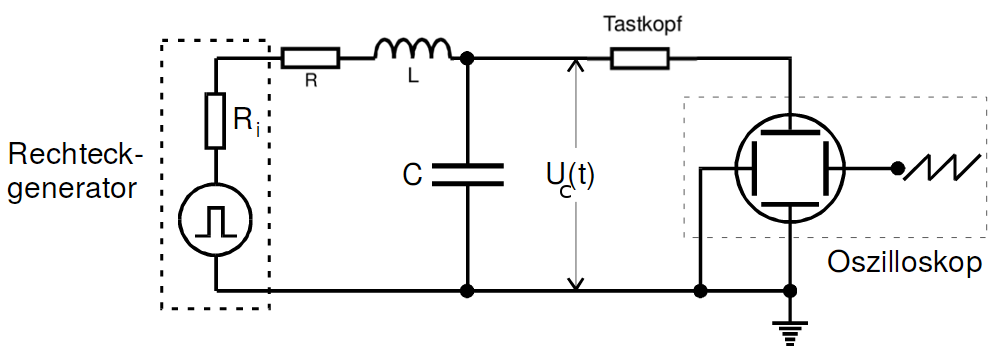
\includegraphics[width=\linewidth-200pt,height=\textheight-200pt,keepaspectratio]{content/images/Aufgabea.png}
\caption{Versuchsaufbau für den ersten Teilversuch \cite{V354}.}
\label{fig:Aufgabea}
\end{figure}

\subsection{Bestimmung der Frequenzabhängigkeit der Amplitude und der Phasenverschiebung der Kondensatorspannung}

Um die Frequenzabhängigkeit der Amplitude $A_.C$ der Kondensatorspannung zu untersuchen wird die Schaltung nach Abbildung \ref{fig:Aufgabec} aufgebaut. Es wird eine Messreihe für $A_.C$ in Abhängigkeit der Frequenz durchgeführt. Die Frequenzabhängigkeit der Generatorspannung $U$ wird überprüft und notiert. Die Güte $q$ und die Breite $B$ werden mittels einer Ausgleichsrechnung bestimmt.

\begin{figure}
\centering
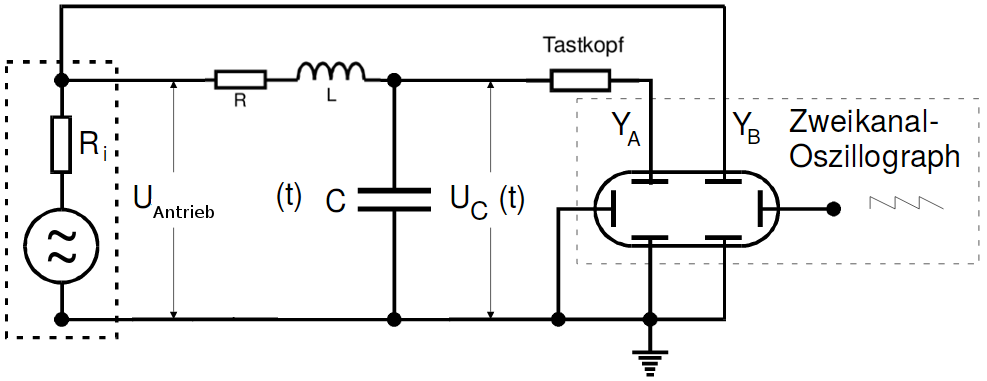
\includegraphics[width=\linewidth-200pt,height=\textheight-200pt,keepaspectratio]{content/images/Aufgabec.png}
\caption{Versuchsaufbau für den dritten Teilversuch \cite{V354}.}
\label{fig:Aufgabec}
\end{figure}

\noindent Für die Phasenverschiebung $\phi$ zwischen Kondensator- und Generatorspannung wird zusätzlich die Generatorspannung über das Oszilloskop ausgegeben. Die Abstände $\Delta t$ der Maxima der übereinander liegenden Graphen werden in Abhängigkeit der Frequenz notiert. Mittels einer Ausgleichsrechnung werden die Resonanzfrequenz $\omega_.{res}$ und die Frequenzen $\omega_.{1,2}$ aus Abschnitt \ref{subsec:RLCPeriodischAngeregt} bestimmt.